%----------------------------------------------------------------------------------------
%	APPENDIX : FOCUS SURFACES
%----------------------------------------------------------------------------------------
%\section{Reconstruction of the focal surfaces}
%\label{sec:focus_surfaces}

Owing to the NIKA2 $6.5~\rm{arcmin}$ FOV, the focus is expected to
slightly change across the FOV, defining curved focal surfaces at the
location of the three arrays. Therefore, beam patterns are expected to
show some scatter across the FOV accordingly to the focal
surfaces. Although all the detectors on a flat array cannot be
individually focalized, an optimal axial focus of the telescope can be
found to maximize the number of detectors at the best focus and hence,
maximize the resolution of the NIKA2 maps.
This optimal focus setting is obtained by measuring the focus at the
center of the arrays as described Sect.~\ref{se:axial_focus} and apply
a focus shift of $-0.2\,\rm{mm}$, which is 
predicted using ZEMAX simulations, and verified by measuring
the focus surfaces as described in the following.

\begin{figure*}[!thbp]
\begin{center}
  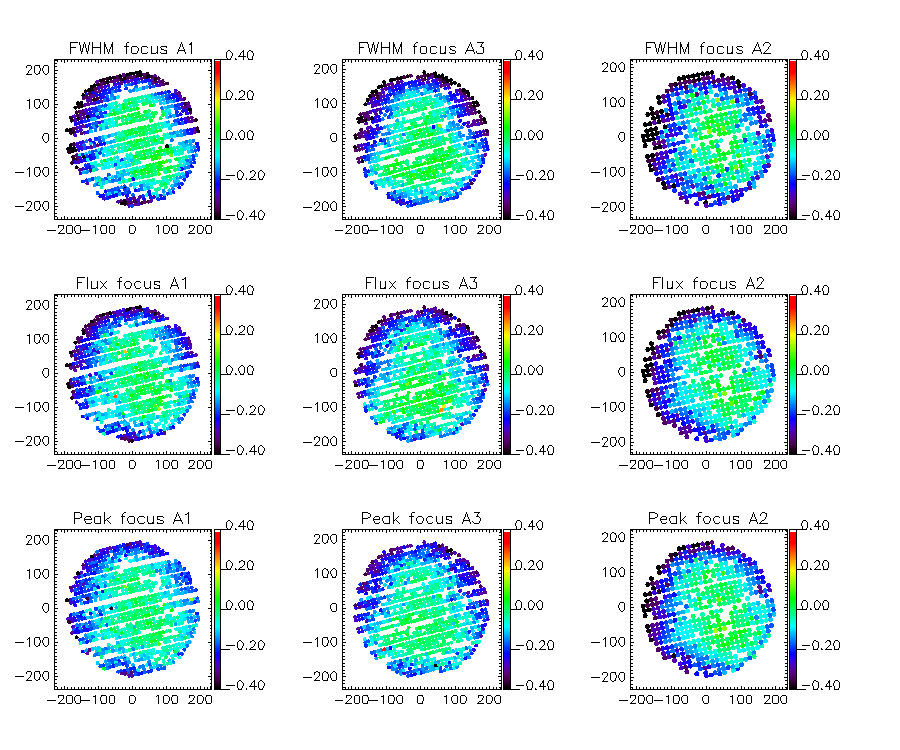
\includegraphics[trim={0, 9.5cm, 0, 9.5cm}, clip=true, width=\linewidth]{Figures/fov_focus_mv_5.png}
\caption[Focus surfaces]{Focus surface of A1, A3 and A2 arrays from left to
  right. In this example, the focus estimates rely on the maximisation of the flux
  density. On each plot, the x and y axis are the Nasmyth offsets
  w.r.t. the center of the array in arcsec, while the color-code represents
  the relative focus estimate w.r.t. the central focus, given in mm.}
\label{fig:focus-surfaces}
\end{center}
\end{figure*}

\subsection{Method}

We estimate NIKA2 focal surfaces by means of a sequence of five \bms\ of bright
point-like sources, typically planets or bright quasars, for various
axial positions $z$ of the telescope sub-reflector around its nominal
position, which is the optimal axial focus $z_{\rm{opt}}$. 
The axial position is changed in step of $0.6~\rm{mm}$ to probe a large
focus range for measuring even the extreme variation of the focus surfaces,
namely $z \in \{-1.2, -0.6, 0, 0.6, 1.2 \} + z_{\rm{opt}}$.  Each
\bm\ is analysed using the data reduction pipeline, as described in
Sect.~\ref{se:dataproc}, and $4''$-resolution individual maps per KID
are produced. 
Therefore, a series of
five maps at various focus positions is available for each detector, from which
the best focus is estimated as described in Sect.~\ref{se:axial_focus}. The
ensemble of the relative focus estimate per KIDs with respect to the best focus
at the center of the array constitutes the focus surface. An accurate estimate
of the center focus is obtained as the weighted average focus estimate of the
KIDs lying in a $30''$ radius around the geometrical center of the array. This
average does not induce any sizeable bias thanks to the flatness of the focus
surface in the innermost regions. For robustness test, we consider three focus
estimates: the first two are the same as discussed in
Sect.~\ref{se:axial_focus} -- namely i) $\hat z_{\rm{fwhm}}$ the focus that
minimizes the geometrical FWHM and ii) $\hat z_{\rm{peak}}$ the focus that
maximizes the amplitude of the best-fitting elliptical Gaussian -- whereas the
third one is $\hat z_{\rm{flux}}$ the focus that maximizes the flux
density in the reference photometric system
(Sect.~\ref{se:photometric_system}). The comparison between the two
estimators based on Gaussian-amplitude fitting ($\hat z_{\rm{peak}}$
and $\hat z_{\rm{flux}}$), will test the stability of the focus
results against the exact choice of the beam fitting function.
%Since
%the ellipticity-based estimator $\hat z_{\rm{ellip}}$ is less
%sensitive to focus changes and yields larger uncertainties than the
%others, we do not use it for the focus surface reconstruction.


\subsection{Data set}

%After the change of A1 lens and the improvement of internal optics
%alignment (hence in the final NIKA2 optical configuration) that is
%during the N2R8 two-day run, N2R9 and N2R10,
%In the final NIK2 optical configuration, 
Nine defocused \bm\ sequences have been acquired, including incomplete
sequences and sequences hindered by poor atmospheric conditions. To
check for systematic effect, a focus measurement is performed
immediately before and after the \bm\ sequence. Using these
measurements, the central focus drift between the starting time and the
end of the sequence is estimated. 
We select sequences that i) comprises at least four scans (four
z-focus steps), ii) have been observed with a zenith opacity at $225\,\rm{GHz}$ (as indicated by
the IRAM \taumeter) below 0.5 and iii) have a maximum central focus
drift of $0.5~\rm{mm}$. These criteria preserve five sequences from which focus
surfaces can be reconstructed, %. Namely, we consider the sequences
%$20170226s415\mbox{--}419$, $20170419s133\mbox{--}137$, $20170420s113\mbox{--}117$,
%$20170421s160\mbox{--}164$ and $20170424s123\mbox{--}127$, which consist of observations
%of the bright quasar 3C84 and Neptune.
corresponding to observations of the bright quasar 3C84 and Neptune.

\subsection{Results}
For each detector $k$ and for each \bm\ sequence $s$, we obtain for
the array $\nu$, a focus measurement $z_\nu^{k, s} \pm \sigma_\nu^{k, s}$,
where $\sigma_\nu^{k, s}$ is the $1\mbox{--}\sigma$ error of the least-square
polynomial fit. The focus surface measurements per array are obtained
as weighted averages of the five \bm\ sequences as in the
following:
%
\begin{equation}
\label{eq:mv_focus_surf}
z_\nu^{(k)} = \left( \sigma_\nu^{(k)} \right)^2 \,  \sum_s \frac{z_\nu^{k,s}}{\left(\sigma_\nu^{k,s}\right)^2}\, \,  ,
\end{equation}
with uncertainties 
\begin{equation}
\label{eq:error_mv_focus_surf}
\sigma_\nu^{(k)} = \left[ \sum_s \frac{1}{\left(\sigma_\nu^{k,s}\right)^2}\right]^{-1/2}\, .
\end{equation}


We present NIKA2 focus surfaces per array obtained as in
Eq.~\ref{eq:mv_focus_surf} for the method of flux density maximization  
%from the inverse-variance weighted combination of the five
%reconstructed focus surfaces per arrays
in Fig.~\ref{fig:focus-surfaces}.
We further check that the three flavours of focus-estimators provide
us with focus surfaces per array that are in good agreement with each
others. Furthermore, they have a non-axisymmetrical flatten bowl
shape, which is well consistent with expectations from optical
simulation using ZEMAX but with slightly higher curvature amplitude.
Namely, the median defocus (that is the relative focus w.r.t. the
central focus) across the detectors is about
$-0.1~\rm{mm}$ for the three arrays. Maximum defocus values of about
$-0.6~\rm{mm}$ are found for detectors corresponding to the outer top and
left regions of the FOV.

We estimate the uncertainty of the focus
surface measurements using the standard deviation between the three
estimators $z_\nu^{(k)}|_{\rm{fwhm}}$, $z_\nu^{(k)}|_{\rm{peak}}$ and
$z_\nu^{(k)}|_{\rm{flux}}$. We found approximatively homogeneous
standard deviation across the FOV with median values of about
$0.03~\rm{mm}$. We also verified the stability of the focus surfaces by comparing
results from a series of \bm\ sequences acquired at various dates and
under various atmospheric conditions.

 %Finally, a fraction comprised between $20$
%and $30\%$ of the KIDs has $z\le -0.2~\rm{mm}$.
{\lp In addition, using optical simulation, we have found that the
variations of beam aberrations are much smaller than the
diffraction pattern, resulting in a quasi invariant beam for a
wide range of defocus up to about $0.3\, \rm{mm}$ around the optimal
focus. For larger defocus, however, the beam starts to deteriorate in
some region of the image plane.}
{\lp Using the results from the measurements and the optical
simulation, we optimize the focus of all detectors by setting the
focus at the value estimated at the center of the arrays shifted of
$-0.2\,\rm{mm}$.}

%Moreover, we cross-check this error estimate by forming the quadratic mean of
%the three inverse-variance error surfaces per array, which are defined in
%Eq.~\ref{eq:error_mv_focus_surf} and quoted
%$\sigma_\nu^{(k)}|_{\rm{fwhm}}$, $\sigma_\nu^{(k)}|_{\rm{peak}}$ and
%$\sigma_\nu^{(k)}|_{\rm{flux}}$. This provides us with more optimistic
%error surfaces per array, which do not show any clear pattern across
%the FOV and which have a median value across the detectors of about
%$0.02~\rm{mm}$. 

%[EXPAND THE DISCUSSION ON COMPARISON WITH SIMULATION]

%\subsection{Focus consistency between arrays}

%\todo{plot de recap sur les differences de focus optimaux observes sur les
%  differents arrays}

%\addparag{summary}
